\documentclass{article}
\usepackage{geometry}
\usepackage{fancyhdr}
\usepackage{amsmath ,amsthm ,amssymb}
\usepackage{graphicx}
\usepackage{hyperref}

% Eigene Makros
\DeclareMathOperator{\diag}{\mathrm{diag}}
\newcommand{\partiell}[3][]{\frac{\partial^{#1}#2}{\partial{#3}^{#1}}}
\newcommand{\diff}[3][]{\frac{\mathrm{d}^{#1}#2}{\mathrm{d}{#3}^{#1}}}
\newcommand{\dr}{\mathrm{d}}
\newcommand{\vect}[1]{\boldsymbol #1}
\newcommand{\Reals}{\mathds R}
\newcommand{\Compl}{\mathds C}
\DeclareMathOperator{\Real}{\mathfrak R}
\DeclareMathOperator{\Imag}{\mathfrak I}
\newcommand{\norm}[1]{\left\|#1\right\|}
\newcommand{\abs}[1]{\left|#1\right|}
\newcommand{\skalprod}[2]{\langle#1,#2\rangle}
\DeclareMathOperator{\grad}{\mathrm{grad}}
\renewcommand{\div}{\mathrm{div}}

\title{Oberseminar Regelungstechnik \\ Regler- und Kalmanfilterentwurf für einen Helikopterversuchstand}
\author{Tilo Stock, Clemens Bilsing, Robert Heedt}
\date {23.11.2018}
\begin{document}
	\maketitle
	\tableofcontents
	\newpage
	\section{Modellbildung}
	Zur Modellbildung des Systems wurde der Lagrange-Formalismus zweiter Art angewendet. Für Systeme mit generalisiertem Potential lautet die Lagrange Gleichung 
	\begin{equation}
	L = T -V
	\end{equation}
	wobei $T$ jeweils die kinetische und $V$ die potentielle Energie des System bezeichnen.
	Mit der Betrachtung von nicht-konservativen Kräften $Q_i$ ergibt sich die Lagrange-Funktion
	\begin{equation}\label{eq:lagrange}
	\diff{}{t} \partiell{L}{\dot{q_i}} - \partiell{L}{q_i}=Q_i
	\end{equation}
	Wobei das Koordinatensystem des Modells $q_i$ festgelegt wurde als
	\begin{equation}
	q = \begin{pmatrix}
	\varphi\\\varepsilon\\\lambda
	\end{pmatrix}
	\end{equation}
	\subsection{Bestimmung der kinetischen- und potentiellen Energien}
	Zur Bestimmung der kinetischen Energie $T$ wurde die Rotation jeder einzelnen Masse um jede Koordinatenachse betrachtet und aufsummiert.
	\begin{equation}
	\begin{split}
	T&= m_p l_p^2\dot{\varphi}^2 + \frac{1}{2}m_cl_c^2\dot{\varepsilon}^2 
	+ m_p(l_h^2+(l_p\sin \varphi)^2)\dot{\varepsilon}^2\\
	&+ \frac{1}{2} m_c (l_c \cos \varepsilon)^2\dot{\lambda}^2\\
	&+ \frac{1}{2} m_p((l_h \cos \varepsilon +l_p \sin \varphi \sin \varepsilon)^2+(l_p \cos \varphi)^2)\dot{\lambda}^2\\
	&+ \frac{1}{2} m_p((l_h \cos \varepsilon -l_p \sin \varphi \sin \varepsilon)^2+(l_p \cos \varphi)^2)\dot{\lambda}^2
	\end{split}
	\end{equation}
	Was vereinfacht werden kann zu
	\begin{equation}
	\begin{split}
	T&= m_p l_p^2\dot{\varphi}^2 \\
	&+ \frac{1}{2}m_cl_c^2\dot{\varepsilon}^2 
	+ m_p(l_h^2+(l_p\sin \varphi)^2)\dot{\varepsilon}^2\\
	&+ \frac{1}{2} m_c (l_c \cos \varepsilon)^2\dot{\lambda}^2\\
	&+ m_p((l_h \cos \varepsilon)^2 + (l_p \sin \varphi \sin \varepsilon)^2+(l_p \cos \varphi)^2)\dot{\lambda}^2
	\end{split}
	\end{equation}
	Die potentielle Energie $V$ lautet
	\begin{equation}
	V = -m_c l_c g \sin \varepsilon + 2 m_p l_h g \sin \varepsilon
	\end{equation}
	Wodurch sich die Lagrange Funktion $L$ ergibt zu 
	\begin{equation}
	\begin{split}
	L = T - V&= m_p l_p^2\dot{\varphi}^2 + \frac{1}{2}m_cl_c^2\dot{\varepsilon}^2 
	+ m_p(l_h^2+(l_p\sin \varphi)^2)\dot{\varepsilon}^2\\
	&+ \frac{1}{2} m_c (l_c \cos \varepsilon)^2\dot{\lambda}^2\\
	&+ m_p((l_h \cos \varepsilon)^2 + (l_p \sin \varphi \sin \varepsilon)^2+(l_p \cos \varphi)^2)\dot{\lambda}^2\\
	&+ m_c l_c g \sin \varepsilon - 2 m_p l_h g \sin \varepsilon
	\end{split}
	\end{equation}
	\subsection{Bestimmung der nicht-konservativen Kräfte}
	Die durch die Rotation der Rotoren sowie durch Gleitreibung entstehen nicht-konservative Kräfte, welche wie folgt vereinfacht\footnote{Die Darstellung von $Q_e$ und $Q_\lambda$ ist vereinfacht worden, damit $(F_f + F_b)$ ausgeklammert werden konnte.} dargestellt werden können:
	\begin{align}
	Q_\varphi &= (F_f - F_b)l_p - \mu_\varphi \dot{\varphi} \\
	Q_\varepsilon &= (F_f + F_b)l_h  \cos \varphi - \mu_\varepsilon \dot{\varepsilon}\\
	Q_\lambda &= (F_f + F_b)l_h \cos \varepsilon \sin \varphi - \mu_\lambda \dot{\lambda}
	\end{align}
	\subsection{Aufstellen der Bewegungsgleichung um $\varphi$}
	\begin{align}
	\partiell{L}{\dot{\varphi}} &= 2m_p l_p^2 \dot{\varphi}\\
	\diff{}{t} \partiell{L}{\dot{\varphi}} &= 2m_p l_p^2 \ddot{\varphi}
	\end{align}
	\begin{equation}
	\begin{split}
	\partiell{L}{\varphi} &= \partiell{}{\varphi} (m_p l_p^2 \dot{\varepsilon}^2 \sin^2 (\varphi) 
	+ m_p l_p^2 \sin^2 (\varepsilon) \dot{\lambda}^2 \sin^2 (\varphi)
	+ m_p l_p^2 \dot{\lambda}^2 \cos^2 \varphi)\\
	&= 2 m_p l_p^2 \dot{\varepsilon}^2 \cos \varphi \sin \varphi + 2 m_p l_p^2 \sin^2 (\varepsilon) \dot{\lambda}^2 \cos \varphi \sin \varphi 
	- 2 m_p l_p^2 \dot{\lambda}^2 \cos \varphi \sin \varphi\\
	&= 2 m_p l_p^2 \cos \varphi \sin \varphi (\dot{\varepsilon}^2+ \sin^2 (\varepsilon) \dot{\lambda}^2- \dot{\lambda}^2)\\
	&= 2 m_p l_p^2 \cos \varphi \sin \varphi (\dot{\varepsilon}^2- \cos^2 (\varepsilon) \dot{\lambda}^2)
	\end{split}
	\end{equation}
	Eingesetzt in \eqref{eq:lagrange} ergibt:
	\begin{equation}
	\underbrace{2m_p l_p^2}_{J_\varphi} \ddot{\varphi} -  \underbrace{2 m_p l_p^2}_{J_\varphi} \cos (\varphi) \sin (\varphi) (\dot{\varepsilon}^2- \cos^2 (\varepsilon) \dot{\lambda}^2) = (F_f - F_b)l_p - \mu_\varphi \dot{\varphi} = V_d \underbrace{K_f l_p}_{L_1} - \mu_\varphi \dot{\varphi}
	\end{equation}
	\subsection{Aufstellen der Bewegungsgleichung um $\varepsilon$}
	\begin{equation}
	\partiell{L}{\dot{\varepsilon}} = 2(\frac{1}{2}m_cl_c^2
	+ m_p(l_h^2+(l_p\sin \varphi)^2))\dot{\varepsilon}
	\end{equation}
	\begin{equation}
	\diff{}{t}\partiell{L}{\dot{\varepsilon}} = (m_cl_c^2
	+ 2 m_p(l_h^2+l_p^2\sin^2 \varphi))\ddot{\varepsilon}
	\end{equation}
	\begin{equation}
	\begin{split}
	\partiell{L}{\varepsilon} &= \partiell{}{\varepsilon}(\frac{1}{2} m_c l_c^2 \dot{\lambda}^2 \cos^2 (\varepsilon) + m_p \dot{\lambda}^2 (l_h^2 \cos^2 (\varepsilon) + l_p^2 \sin^2 (\varphi) \sin^2 (\varepsilon))
	+ m_c l_c g \sin \varepsilon - 2 m_p l_h g \sin \varepsilon)\\
	&= -m_c l_c^2 \dot{\lambda}^2 \cos \varepsilon \sin \varepsilon + 2 m_p \dot{\lambda}^2 \cos \varepsilon \sin \varepsilon (-l_h^2  + l_p^2 \sin^2 (\varphi) ) + g(m_c l_c - 2 m_p l_h) \cos \varepsilon\\
	&= \cos \varepsilon \sin \varepsilon  (-m_c l_c^2 + 2 m_p (l_p^2 \sin^2 (\varphi) -l_h^2  )) \dot{\lambda}^2+ g(m_c l_c - 2 m_p l_h) \cos \varepsilon
	\end{split}
	\end{equation}
	Eingesetzt in \eqref{eq:lagrange} ergibt:
	\begin{equation}
	\begin{split}
	&(m_cl_c^2+ 2 m_p(l_h^2+l_p^2\sin^2 \varphi))\ddot{\varepsilon} - \cos \varepsilon \sin \varepsilon (-m_c l_c^2 + 2 m_p (l_p^2 \sin^2 (\varphi) -l_h^2  ))\dot{\lambda}^2 \\
	& - g(m_c l_c - 2 m_p l_h) \cos \varepsilon = (F_f + F_b)l_h  \cos \varphi - \mu_\varepsilon \dot{\varepsilon}
	\end{split}
	\end{equation}
	
	\begin{equation}
	\begin{split}
	&\overbrace{(m_cl_c^2+ 2 m_p(l_h^2+l_p^2\sin^2 \varphi))}^{J_\varepsilon}\ddot{e} + \cos \varepsilon \sin \varepsilon \overbrace{(m_c l_c^2 + 2 m_p ( l_h^2 -l_p^2 \sin^2 (\varphi) ))}^{\approx J_\varepsilon} \dot{\lambda}^2 \\
	&= \underbrace{g(m_c l_c - 2 m_p l_h)}_{L_2} \cos \varepsilon + V_s \underbrace{ K_f l_h}_{L_3}  \cos \varphi  - \mu_\varepsilon \dot{\varepsilon}
	\end{split}
	\end{equation}
	\begin{figure}[ht]
		\centering
		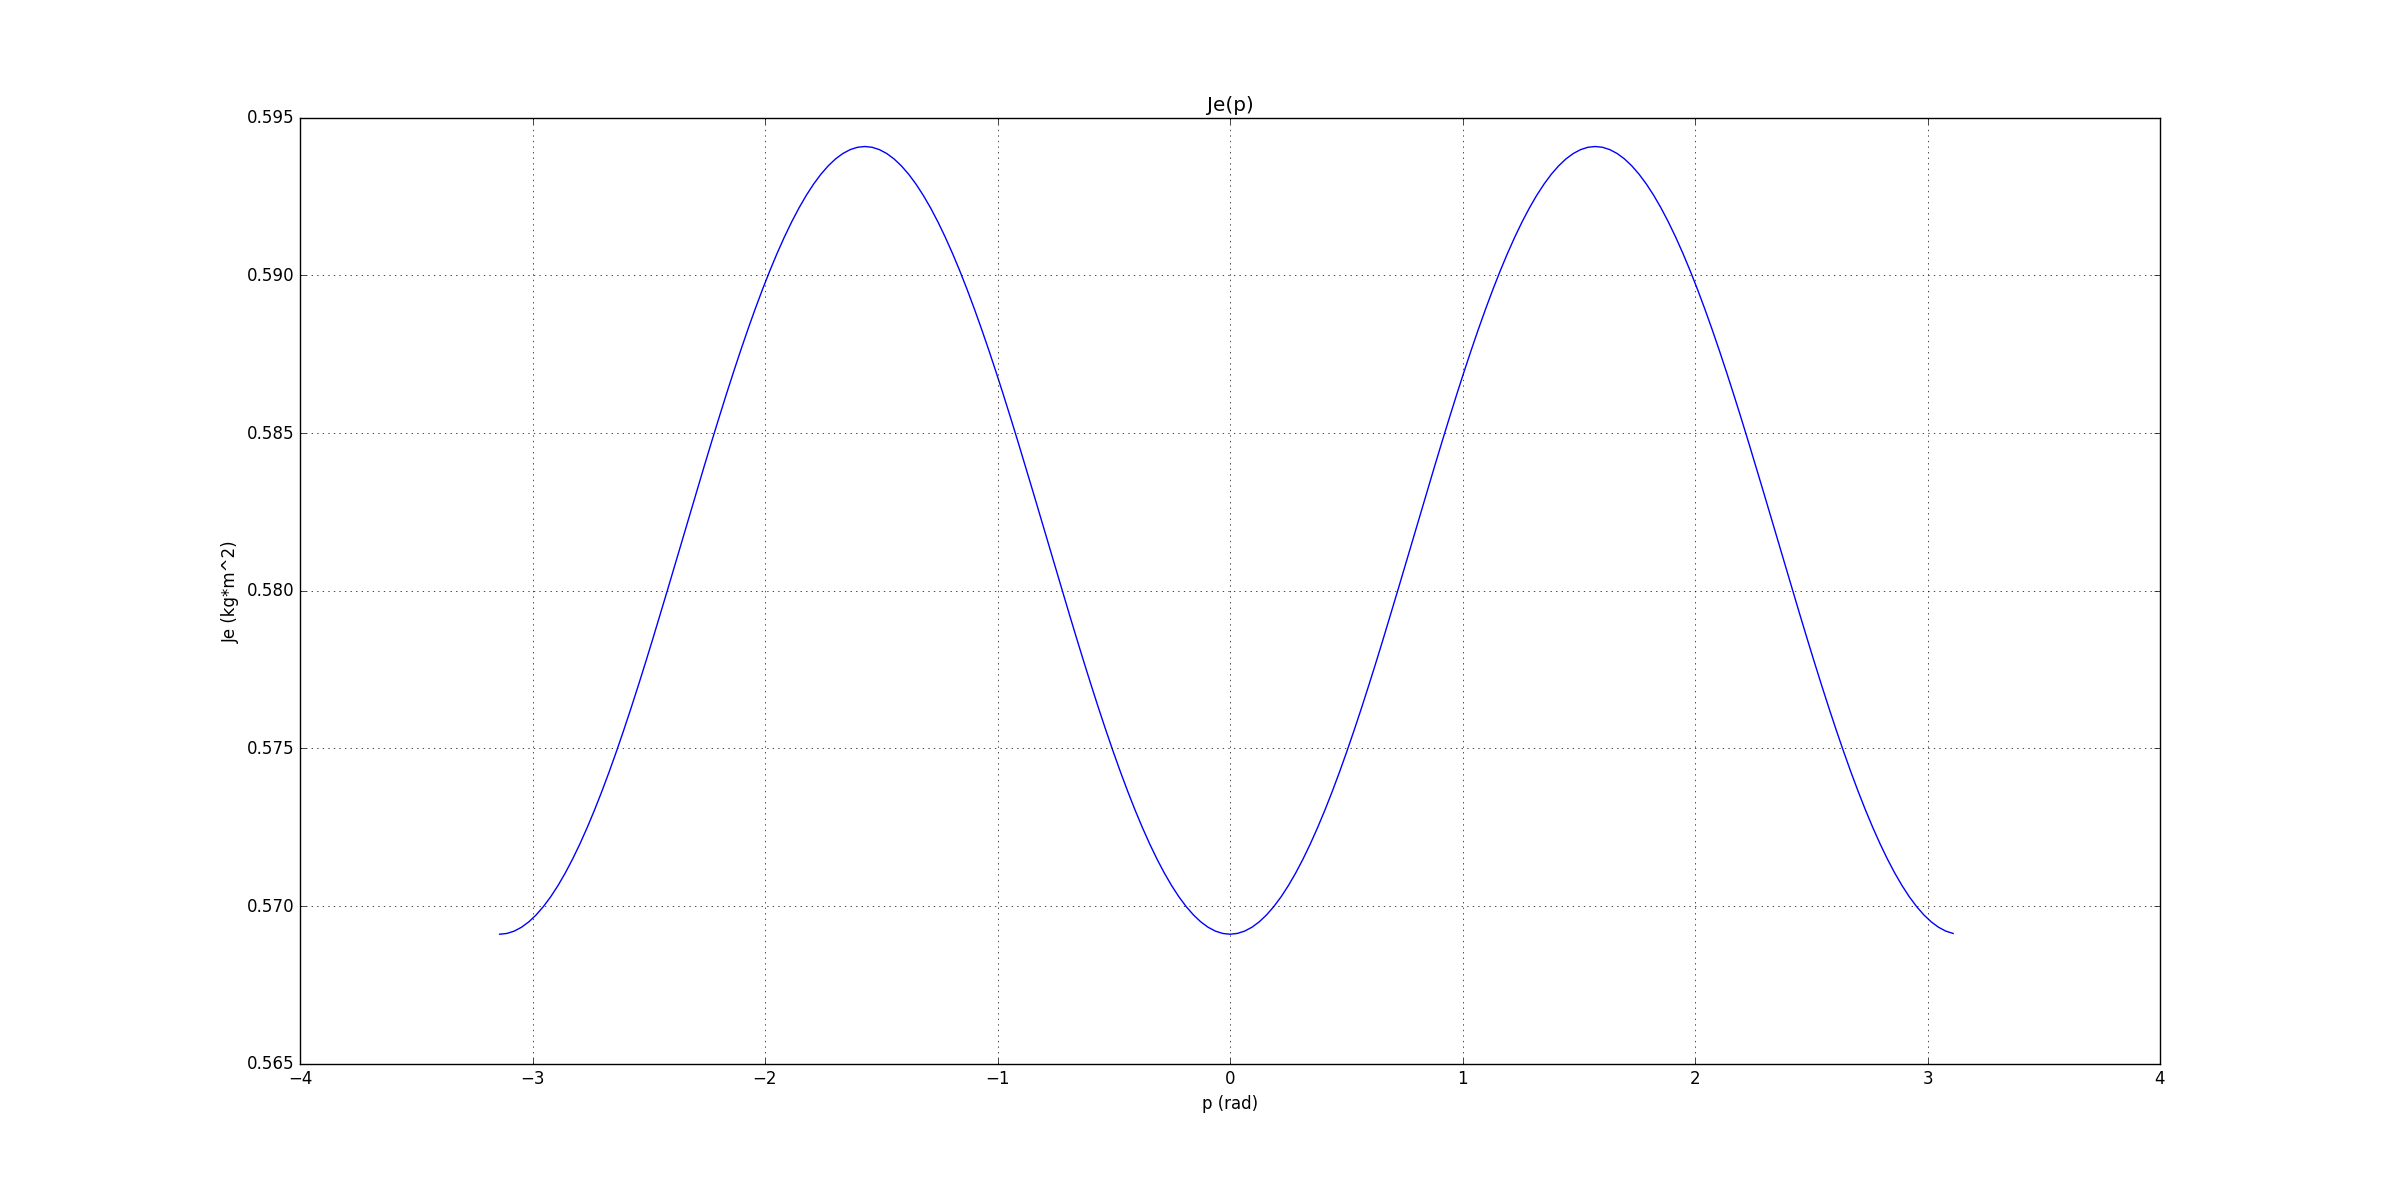
\includegraphics[width=1\textwidth]{images/J_e}
		\caption{$J_\varepsilon(\varphi)$ in Abhängigkeit des Winkels $\varphi$}
		\label{fig:J_e}
	\end{figure}
	\subsection{Aufstellen der Bewegungsgleichung um $\lambda$}
	\begin{equation}
	\partiell{L}{\dot{\lambda}} = (m_c (l_c \cos \varepsilon)^2
	+ 2 m_p((l_h \cos \varepsilon)^2 + (l_p \sin \varphi \sin \varepsilon)^2+(l_p \cos \varphi)^2))\dot{\lambda}
	\end{equation}
	\begin{equation}
	\diff{}{t}\partiell{L}{\dot{\lambda}} = (m_c (l_c \cos \varepsilon)^2
	+ 2 m_p((l_h \cos \varepsilon)^2 + (l_p \sin \varphi \sin \varepsilon)^2+(l_p \cos \varphi)^2))\ddot{\lambda}
	\end{equation}
	\begin{equation}
	\partiell{L}{\lambda} = 0
	\end{equation}
	Eingesetzt in \eqref{eq:lagrange} ergibt:
	\begin{equation}
	\underbrace{(m_c (l_c \cos \varepsilon)^2
	+ 2 m_p((l_h \cos \varepsilon)^2 + (l_p \sin \varphi \sin \varepsilon)^2+(l_p \cos \varphi)^2))}_{J_\lambda}\ddot{\lambda} =  V_s \underbrace{K_f l_h}_{L_4} \cos \varepsilon \sin \varphi - \mu_\lambda \dot{\lambda}
	\end{equation}
	\begin{figure}[ht]
		\centering
		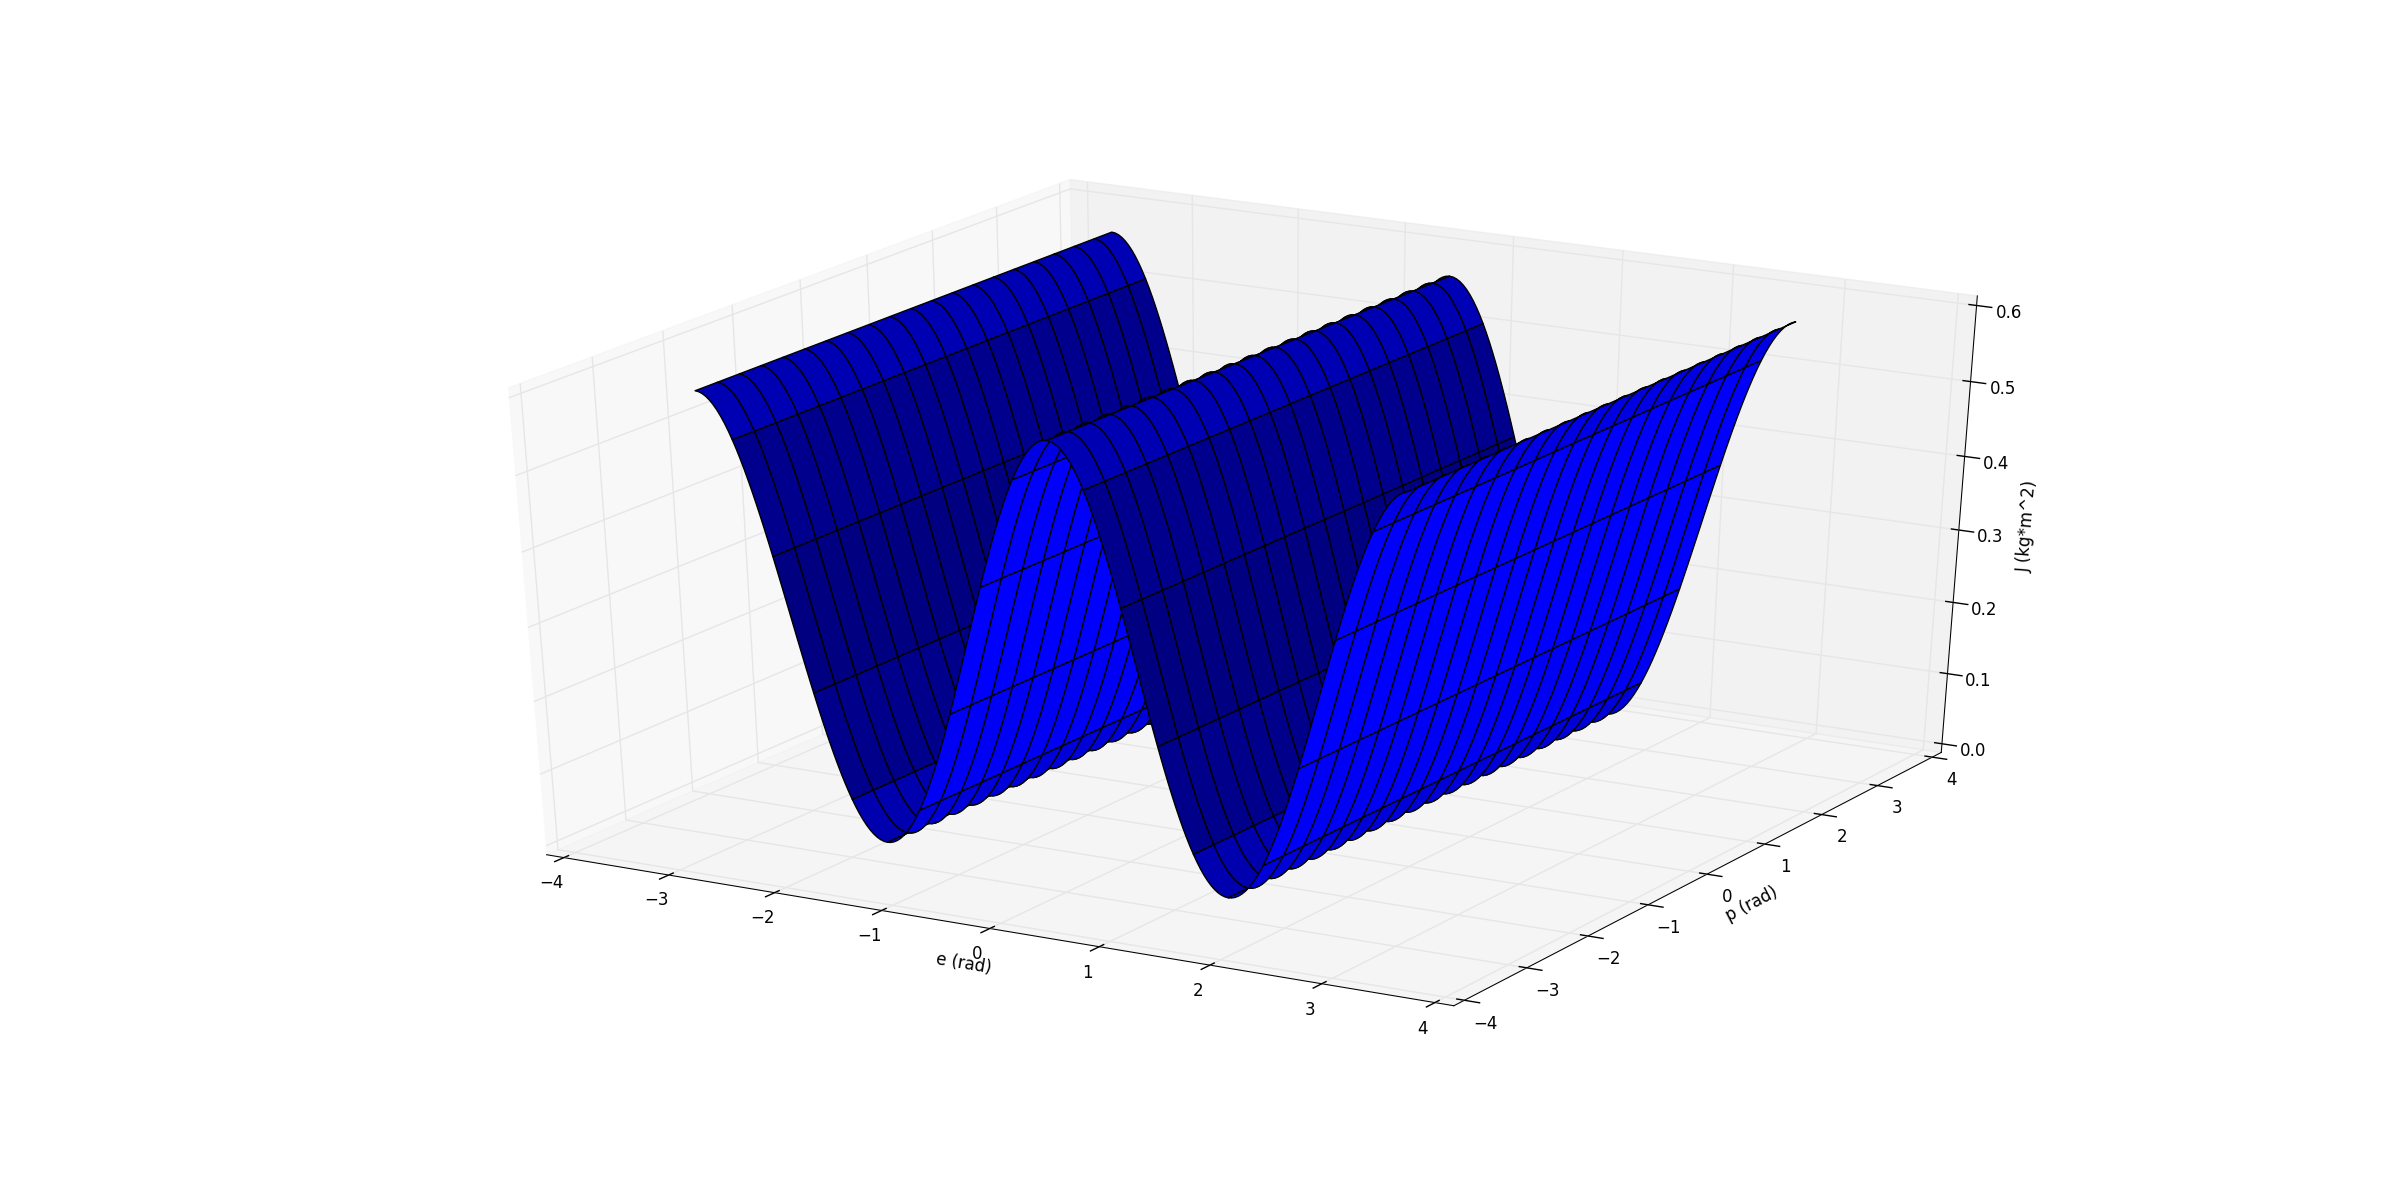
\includegraphics[width=1\textwidth]{images/J_l}
		\caption{$J_\lambda(\varepsilon,\varphi)$ in Abhängigkeit der Winkel $\varphi$ und $\varepsilon$}
		\label{fig:J_l}
	\end{figure}	
	\subsection{Zusammenfassen der Bewegungsgleichungen}
	Insgesamt kann das System mit wie folgt dargestellt werden:
	\begin{align}
	J_\varphi \ddot{\varphi} + \mu_\varphi \dot{\varphi} - J_\varphi \cos (\varphi) \sin (\varphi) (\dot{\varepsilon}^2- \cos^2 (\varepsilon) \dot{\lambda}^2) &= V_d L_1\\
	J_\varepsilon(\varphi)\ddot{\varepsilon} + \mu_\varepsilon \dot{\varepsilon} + J_\varepsilon(\varphi) \cos (\varepsilon) \sin (\varepsilon) \dot{\lambda}^2 
	&= L_2 \cos \varepsilon + V_s L_3 \cos \varphi\\
	J_\lambda(\varepsilon,\varphi) \ddot{\lambda} + \mu_\lambda \dot{\lambda} &= V_s L_4 \cos \varepsilon \sin \varphi
	\end{align}
	Mit $J_\varepsilon(\varphi)$ und $	J_\lambda(\varepsilon,\varphi)$ zu:
	\begin{align}
	J_\lambda(\varepsilon,\varphi) &= m_c (l_c \cos \varepsilon)^2
	+ 2 m_p((l_h \cos \varepsilon)^2 + (l_p \sin \varphi \sin \varepsilon)^2+(l_p \cos \varphi)^2)\\
	J_\varepsilon(\varphi) &= m_cl_c^2+ 2 m_p(l_h^2+l_p^2\sin^2 \varphi)
	\end{align}
	\subsection{Erweiterung des Systems durch Rotordrehzahlen}
	Die Kraft jedes Rotors resultiert nun aus der Drehzahl jedes Motors, wobei diese durch einen Tiefpass 1. Ordnung beschrieben werden können.
	\begin{align}
	T_f \dot{\omega_f} + \omega_f &= K_f V_f\\
	T_b \dot{\omega_b} + \omega_b &= K_b V_b
	\end{align}
	Dabei beschreibt $\omega_f$ und $\omega_b$ die Drehzahl der beiden Motoren und $T_f$ sowie $T_b$ deren Zeitkonstante.
	Damit kann die auf das System resultierende Kraft beschrieben werden durch:
	\begin{equation}
	F_s = F_f + F_b = K (\omega_f + \omega_b)
	\end{equation}
	\begin{equation}
	F_b = F_f - F_b = K (\omega_f - \omega_b)
	\end{equation}
	Weiterhin entstehen aus der Rotordrehzahl das jeweiliges Drehmoment $M_f$ und $M_b$ der Elektromotoren. Diese bewirken ein zusätzliches Moment auf die Drehachse um $\varepsilon$ und $\lambda$.
	\begin{align}
	M_{M,\varepsilon} &= \sin (\varphi) (M_f - M_b) =\sin (\varphi) K_M (\omega_f-\omega_b) \\
	M_{M,\lambda} &= \cos (\varepsilon) \cos (\varphi) (M_b - M_f) =\cos (\varepsilon) \cos (\varphi) K_M (\omega_b-\omega_f)
	\end{align}
	Das resultierende System ist daher:
	\begin{align}
	&J_\varphi \ddot{\varphi} + \mu_\varphi \dot{\varphi} - J_\varphi \cos (\varphi) \sin (\varphi) (\dot{\varepsilon}^2- \cos^2 (\varepsilon) \dot{\lambda}^2) = K l_p (\omega_f - \omega_b)\\
	&J_\varepsilon(\varphi)\ddot{\varepsilon} + \mu_\varepsilon \dot{\varepsilon} + J_\varepsilon(\varphi) \cos (\varepsilon) \sin (\varepsilon) \dot{\lambda}^2 
	= L_2 \cos \varepsilon + K l_h \cos \varphi (\omega_f + \omega_b) + \sin (\varphi) K_M (\omega_f-\omega_b)\\
	&J_\lambda(\varepsilon,\varphi) \ddot{\lambda} + \mu_\lambda \dot{\lambda} = K l_h \cos \varepsilon \sin \varphi (\omega_f + \omega_b) +\cos (\varepsilon) \cos (\varphi) K_M (\omega_b-\omega_f)
	\end{align}
	\subsection{Erweiterung des Systems durch Kreiselträgheit}
	Zusätzlich wirken Kreiselmomente auf die Rotoren, wenn sich die Rotationsachse der Rotoren verändert. Diese Kreiselmomente können allgemein beschreiben werden durch:
	\begin{equation}
	\vec{M} = \vec{\Omega} \times \vec{L}
	\end{equation}	
	Angewandt auf Rotation um $\varphi$:
	\begin{align}
	&M_{K\varepsilon,\varphi} = J_M \cos (\varphi) \dot{\varphi}(\omega_f-\omega_b)\\
	&M_{K\lambda,\varphi} = J_M \sin (\varphi) \cos (\varepsilon) \dot{\varphi}(\omega_f-\omega_b)
	\end{align}
	Angewandt auf Rotation um $\varepsilon$:
	\begin{equation}
	M_{K\varphi,\varepsilon} = J_M \cos (\varphi) \dot{\varepsilon}(\omega_b-\omega_f)
	\end{equation}
	Angewandt auf Rotation um $\lambda$:
	\begin{align}
	&M_{K\varphi,\lambda} = J_M \sin (\varphi) \cos (\varepsilon) \dot{\lambda}(\omega_f-\omega_b)\\
	&M_{K\varepsilon,\lambda} = J_M \cos (\varphi) \sin (\varepsilon) \dot{\lambda}(\omega_b-\omega_f)
	\end{align}
	Das resultierende System ist daher:
	\begin{align}
	&J_\varphi \ddot{\varphi} + \mu_\varphi \dot{\varphi} - J_\varphi \cos (\varphi) \sin (\varphi) (\dot{\varepsilon}^2- \cos^2 (\varepsilon) \dot{\lambda}^2) = K l_p (\omega_f - \omega_b) \\&+  J_M \cos (\varphi) \dot{\varepsilon}(\omega_b-\omega_f) +  J_M \cos (\varphi) \sin (\varepsilon) \dot{\lambda}(\omega_b-\omega_f)  
	\end{align}
	\begin{align}
	&J_\varepsilon(\varphi)\ddot{\varepsilon} + \mu_\varepsilon \dot{\varepsilon} + J_\varepsilon(\varphi) \cos (\varepsilon) \sin (\varepsilon) \dot{\lambda}^2 = L_2 \cos \varepsilon + K l_h \cos \varphi (\omega_f + \omega_b) \\
	&+ \sin (\varphi) K_M (\omega_f-\omega_b)+  J_M \cos (\varphi) \dot{\varphi}(\omega_f-\omega_b) +J_M \cos (\varphi) \sin (\varepsilon) \dot{\lambda}(\omega_b-\omega_f)
	\end{align}
	\begin{align}
	J_\lambda(\varepsilon,\varphi) \ddot{\lambda} + \mu_\lambda \dot{\lambda} = K l_h \cos \varepsilon \sin \varphi (\omega_f + \omega_b) +\cos (\varepsilon) \cos (\varphi) K_M (\omega_b-\omega_f) + J_M \sin (\varphi) \cos (\varepsilon) \dot{\varphi}(\omega_f-\omega_b)
	\end{align}
	%\begin{align}
	%&V_s K_f = F_f + F_b \\
	%&V_d K_f = F_f - F_b
	%\end{align}
	%\begin{align}
	%&\dot{\lambda} = const \\
	%&V_s = 0\\
	%&V_d = 0
	%\end{align}

\end{document}